%(BEGIN_QUESTION)
% Copyright 2009, Tony R. Kuphaldt, released under the Creative Commons Attribution License (v 1.0)
% This means you may do almost anything with this work of mine, so long as you give me proper credit

Acetone -- a valuable industrial solvent (chemical formula C$_{3}$H$_{6}$O) -- may be manufactured from isopropyl alcohol (chemical formula C$_{3}$H$_{8}$O) in a chemical reaction that breaks two atoms of hydrogen away from each molecule of alcohol, leaving acetone and hydrogen gas (H$_{2}$) as byproducts:

$$\hbox{C}_3\hbox{H}_8\hbox{O} \rightarrow \hbox{C}_3\hbox{H}_6\hbox{O} + \hbox{H}_2$$

A simplified flow diagram for this process is shown here:

$$\includegraphics[width=15.5cm]{i04060x01.eps}$$

Suppose the decision is made to use a vortex flowmeter to measure acetone reflux flow into the distillation tower.  This particular vortex flowmeter has a minimum Reynolds number value of 10,000 as specified by the manufacturer.  Calculate the minimum flow rate of acetone at 20 $^{o}$C this vortex meter will be able to measure given a schedule-40 pipe size of 1-1/2 inches (1.610 inches internal diameter).  Assume a density of 49.4 pounds per cubic foot and an absolute viscosity of 0.32 centipoise for acetone at this temperature.

\vskip 20pt \vbox{\hrule \hbox{\strut \vrule{} {\bf Suggestions for Socratic discussion} \vrule} \hrule}

\begin{itemize}
\item{} Why would you as a technician (not an engineer) need to know anything about {\it minimum flow cutoff} for a vortex flowmeter?  Identify a practical scenario where this knowledge might become important for you to do your job.
\item{} Explain what the {\it Reynolds number} of a flowing fluid means in your own words.  Specifically, what effects are manifest from different Reynolds number values?
\item{} What is the purpose of a {\it distillation tower} in this particular process and how does it work?
\item{} If you are familiar with distillation tower operation, identify which sunstance has the lower boiling point: acetone or isopropyl alcohol.
\end{itemize}

\underbar{file i04060}
%(END_QUESTION)





%(BEGIN_ANSWER)


%(END_ANSWER)





%(BEGIN_NOTES)

$$\hbox{Re} = {{3160 G_f Q} \over {D \mu}}$$

\noindent
Where,

Re = Reynolds number (unitless)

$G_f$ = Specific gravity of liquid (unitless)

$Q$ = Flow rate (gallons per minute)

$D$ = Diameter of pipe (inches)

$\mu$ = Absolute viscosity of fluid (centipoise)

3160 = Conversion factor for British units

\vskip 10pt

The specific gravity of this acetone is equal to $49.4 \over 62.4$ = 0.791667, therefore:

$$Q = {D \mu \hbox{Re} \over 3160 G_f} = {(1.610)(0.32)(10000) \over (3160)(0.791667)} = 2.059 \hbox{ GPM}$$

\vskip 10pt

We must have a flow rate of at least 2.059 gallons per minute in order for this vortex flowmeter to operate, and not enter into low-flow cutoff.

\vskip 10pt

Note that the temperature given in the problem does not enter into any calculation for the solution.  However, this does not mean that temperature is irrelevant!  Temperature strongly affects both fluid viscosity and density, and so is very relevant to the problem.

\vskip 10pt

Details on process chemistry taken from page 764 of {\it Shreve's Chemical Process Industries}, fifth edition, by George T. Austin.

%INDEX% Measurement, flow: vortex
%INDEX% Process: acetone production reactor

%(END_NOTES)


